\subsection{选择粒度的受控研究}
\label{sec:fm-granularity-study}
图~\ref{fig:fm-motivation} 的研究将可训练子集决策与评分数据来源区分开来。我们在 CIFAR100/ViT-base 上使用 36 个 Q/K/V 候选、五个客户端、IID 和 Dirichlet-$1.0/0.1$ 划分，以及种子 2024--2026。形成客户端数据前，从训练划分中预留独立的服务器代理样本池和预热数据划分。每个客户端留出 100 个样本用于验证。本地画像使用 16 个客户端训练样本；Proxy 对五个互不重叠、各含 16 个样本的代理批次求平均。两个检查点分别是适配器初始化，以及在独立预留集上预热 100 步后的结果，并非两个联邦通信轮次。

对于每个客户端、检查点和评分来源，矩阵选择器在资源可行的 12 目标子集中最大化画像评分。层选择器枚举所有四块组合，在每个被选块中将 Q/K/V 绑定。两者使用相同的来源评分、深度因子、资源限制和秩 8；LoRA 与共同训练的分类头参数数量相同。在所用资源模型下，全部 360 条方法记录均可行。未选中的适配器保留在前向模型中但被冻结，且每个配置都从相同的验证损失出发。20 步 AdamW 训练使用学习率 $10^{-3}$、每组配对内相同的数据顺序和受控随机状态。这一协议衡量匹配初始函数后的适配效果，而不是删除适配器带来的内存收益。

矩阵--层差值先在每个种子内对五个客户端求平均，再跨三个种子汇总。全部 12 个设置级均值为正；36 个种子内配对均值中有 35 个、180 个客户端级配对中有 161 个偏向矩阵级选择。完整数值汇总见附录~\ref{app:fm-p2-details}。由于两种评分来源下都观察到改进，该研究支持解除完整层绑定，而不要求本地评分优于代理评分。深度校准沿用与方法相同的划分相关日程，并在每组配对内固定。

\subsection{评分可靠性}\label{sec:fm-score-study}
接下来考察可加效用是否能为所选矩阵--层配对之外的配置提供有用的排序信息。在 CIFAR100 研究的每个客户端与检查点上，我们评估原有的 12 个不同的可行配置，其中包含评分引导和随机子集。每个配置均使用 12 个秩为 8 的目标、相同训练长度和匹配的初始适配器。结果指标是在留出本地样本上的训练前损失减去训练后损失。粒度对比新增的层级配置不加入这个候选池。

原始评分和深度校准评分的 Spearman 相关系数分别在每个客户端--检查点候选池内计算。先在每个种子内对五个客户端系数求平均，再报告三个种子的均值和样本标准差。统计使用配对随机状态修复后的训练结果；配置身份和评分值均保持不变。

\newcommand{\FMAdepthMin}{0.657}
\newcommand{\FMAdepthMax}{0.876}
\newcommand{\FMApositive}{90}
\newcommand{\FMAtotal}{90}
\newcommand{\FMAassociationSentence}{这些设置级的正相关支持在本受控协议中使用画像效用为配置确定优先级。}
\begin{table}[t]
\centering
\caption{客户端内部的配置排序可靠性。数值为先对客户端求平均、再跨三个种子计算的 Spearman 系数均值 $\pm$ 样本标准差。预热表示共同的 100 步检查点。}
\label{tab:fm-score-reliability}
\small
\setlength{\tabcolsep}{3pt}
\begin{tabular}{@{}llcc@{}}
\toprule
数据划分 & 状态 & 原始评分 & 校准评分 \\
\midrule
IID & 初始化 & $0.688\pm0.114$ & $0.746\pm0.067$ \\
IID & 预热 & $0.595\pm0.094$ & $0.657\pm0.070$ \\
Dir. $1.0$ & 初始化 & $0.792\pm0.012$ & $0.841\pm0.042$ \\
Dir. $1.0$ & 预热 & $0.556\pm0.141$ & $0.664\pm0.136$ \\
Dir. $0.1$ & 初始化 & $0.885\pm0.028$ & $0.772\pm0.028$ \\
Dir. $0.1$ & 预热 & $0.801\pm0.023$ & $0.876\pm0.036$ \\
\bottomrule
\end{tabular}
\end{table}


校准评分的六个设置级平均相关系数介于 \FMAdepthMin{} 与 \FMAdepthMax{} 之间；\FMAtotal{} 个客户端--检查点系数中有 \FMApositive{} 个为正。\FMAassociationSentence{} 表~\ref{tab:fm-score-reliability} 对相同训练结果报告原始和校准评分，从而区分梯度信号的信息量与位置因子的作用。本实验考察短期配置排序；下一个消融在完整联邦训练中评估这些设计。

\subsection{矩阵级适配的消融}\label{sec:fm-ablations}
我们使用 Dirichlet-$1.0$ 划分下的 SST-2/RoBERTa-base 隔离三个组成部分。Full 与三个变体比较：Server-Proxy 用仅从预留训练样本构建的共享代理评分替代本地评分；Layer-Level 保留本地评分，但绑定同一块中的 Q/K/V 选择；No-Depth 仅移除位置乘子。在每个种子内，所有变体使用相同的私有数据与代理数据划分、秩 8、本地优化器设置、候选客户端协议、资源限制和 80 轮训练长度。实际选中的客户端及目标子集仍是分配结果。三个种子为 2024--2026，每次运行消耗累计 7,200 的矩阵等价预算。该受控研究具有自己的代理预留集，与历史主对比实验分开报告。

\begin{table}[t]
\centering
\caption{累计矩阵等价预算为 7,200 时的 SST-2 组成部分消融。验证准确率以百分比表示，报告三个种子的均值 $\pm$ 样本标准差。最佳值为每次运行中的峰值。粗体表示各指标列的最大均值。}
\label{tab:fm-ablations}
\small
\setlength{\tabcolsep}{4pt}
\begin{tabular}{@{}lcc@{}}
\toprule
变体 & 最终准确率 & 最佳准确率 \\
\midrule
Full & $\mathbf{90.60}\pm0.72$ & $90.87\pm0.50$ \\
Server-Proxy & $90.47\pm0.81$ & $90.80\pm0.87$ \\
Layer-Level & $90.07\pm1.33$ & $90.73\pm0.42$ \\
No-Depth & $90.47\pm0.61$ & $\mathbf{90.93}\pm0.42$ \\
\bottomrule
\end{tabular}
\end{table}

\begin{figure}[t]
\centering
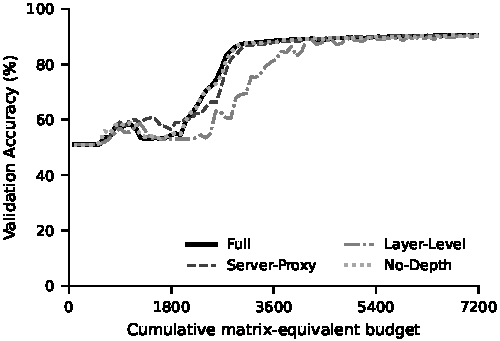
\includegraphics[width=\columnwidth]{figures/fig6_ablation_budget.pdf}
\caption{四种消融变体在完整累计预算轨迹上的三种子平均验证准确率。终点的运行间变化和各运行峰值指标见表~\ref{tab:fm-ablations}。横轴为矩阵等价训练成本，而非实测运行时间。}
\label{fig:fm-ablation-budget}
\end{figure}

表~\ref{tab:fm-ablations} 同时报告最终与最佳准确率，图~\ref{fig:fm-ablation-budget} 展示完整预算轨迹。Full 的最终均值最高，分别比 Server-Proxy、Layer-Level 和 No-Depth 高 $0.13$、$0.53$ 和 $0.13$ 个百分点。在这一设置中，绑定完整层造成的最终均值变化最大，与短期粒度研究互为补充。这些差异相对于不同运行之间的变化幅度较小。本地评估和代理评估的观测均值接近，而 No-Depth 的最佳均值略高，为 $90.93\%$。因此，消融将目标粒度的贡献与评分来源和校准较小的终点影响区分开来，而不把完整框架在主基准上的收益归因于某一个组成部分。
